\begin{problem}{/images/problems/pic.jpg}{Coloring the Map of Iran}This is one of the most important problems in the history of graph theory:
	
What is the minimum number of colors needed to color the provinces of Iran so that no two neighboring provinces have the same color?

\textbf{Additional problems}:
\begin{itemize}
\item What is the size of the largest subset of Iranian provinces that can be colored with 3 colors so that no two neighboring provinces have the same color?
\item Question 1, but what about 2 colors?
\item Question 1, but what about 1 color?
\end{itemize}
(link to the map:  \url{https://skilledup.ir/iran-map/)}

\begin{center}
	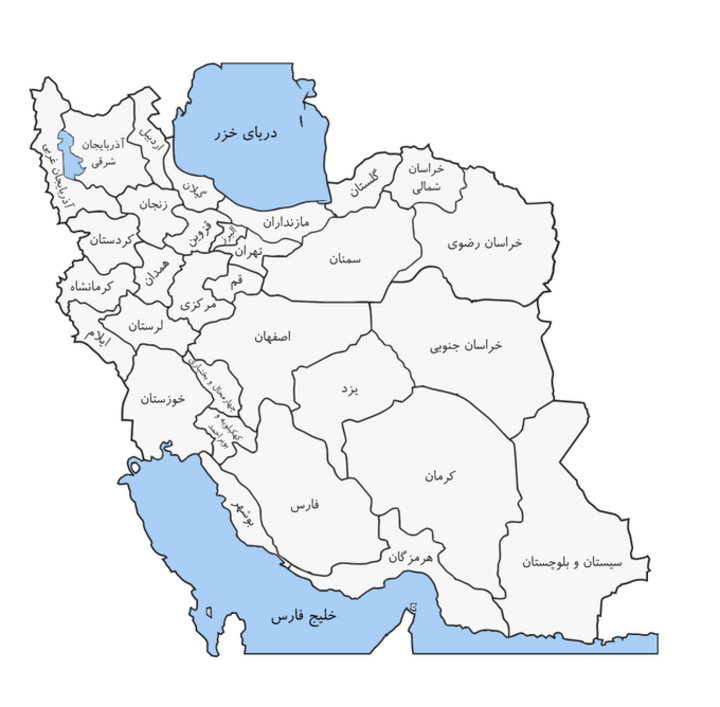
\includegraphics[width=9cm]{/images/problems/43_iran.png}
\end{center}

 Link to the problem on Twitter: \url{https://twitter.com/Riazi_Cafe/status/1707280079318098026}\end{problem}
\begin{solution}
The minimum number of colors for coloring the provinces of Iran is 4. Answers to additional questions: 28 provinces can be colored with 3 colors. 21 provinces can be colored with 2 colors. 12 provinces can be colored with one color. \\[0.2cm]

The map of Iranian cities produces a graph with 31 vertices and the following edges:

\begin{itemize}
	\item $(0, 2), (0, 7), (0, 11), (1, 2), (1, 3), (1, 7), (2, 7), (3, 7), ( 3, 9), (3, 10), (4, 5), (4, 6), (4, 8), (5, 8), (5, 9), (6, 8), (6, 18)$,
	\item $(7, 10), (7, 11), (7, 14), (8, 9), (8, 13), (8, 17), (8, 18), (8, 20) , (9, 10), (9, 12), (9, 13), (10, 12), (10, 14), (10, 15)$, 
	\item $ (11, 14), (11, 16), ( 12, 13), (12, 15), (13, 15), (13, 17), (14, 15), (14, 16), (14, 19), (15, 17), (15, 19), (15, 20), (16, 19)$,
	\item $(16, 21), (17, 20), (18, 20), (18, 22), (18, 25), (18, 27) , (19, 20), (19, 21), (19, 23), (19, 24),(20, 22), (20, 24), (20, 26)$,
	\item $(20, 28), ( 21, 23), (22, 25), (22, 26), (23, 24), (23, 28), (23, 29), (24, 28), (25, 26), (25, 27), (25, 30), (26, 28)$,
	\item $(26, 29), (26, 30), (27, 30), (28, 29), (29, 30)$
\end{itemize}  

\begin{center}
	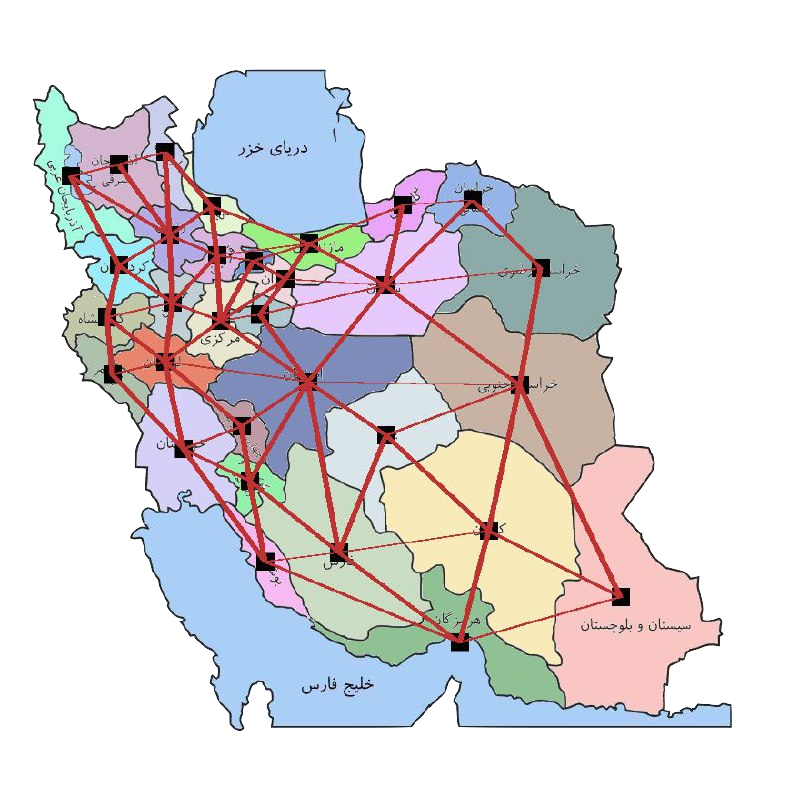
\includegraphics[width=9cm]{/images/problems/43_sol0.png}
\end{center}

The number of colorings with 4 colors is equal to 12427583. An example is given below:

\begin{center}
	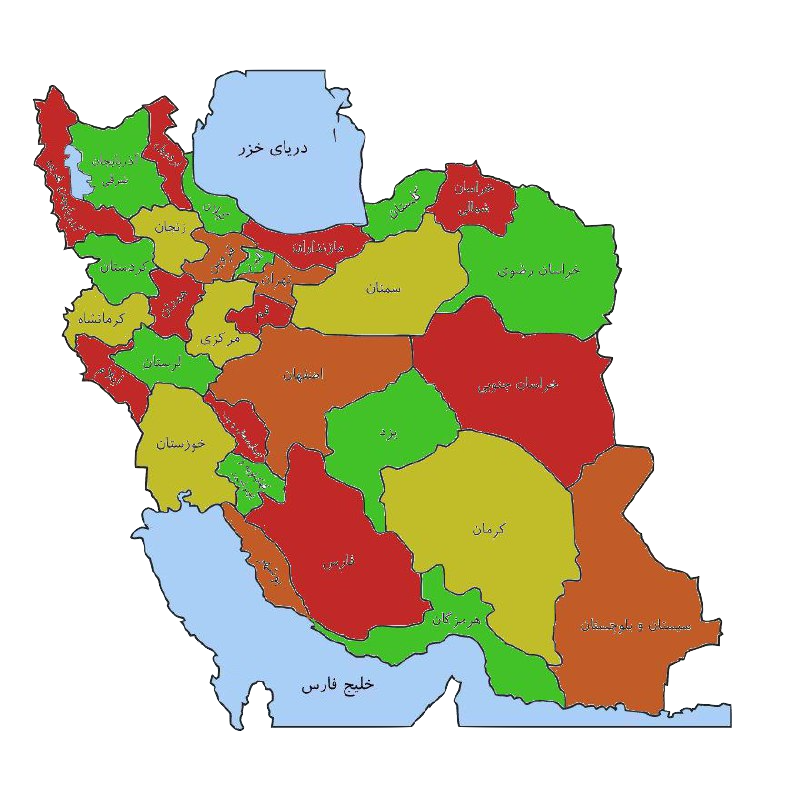
\includegraphics[width=9cm]{/images/problems/43_sol1.png}
\end{center}

The provinces cannot be colored with 3 colors because of the following argument: Some provinces (such as Isfahan) have an odd number of neighbors that are adjacent to each other like a chain, and to paint these neighbors, at least 3 colors are required, and the color of the middle province must be different from these 3 colors.\\[0.2cm]

\textbf{Answers to additional questions}:

It is possible to paint 28 out of 31 provinces in 3 colors so that no neighboring provinces are the same color:

\begin{center}
	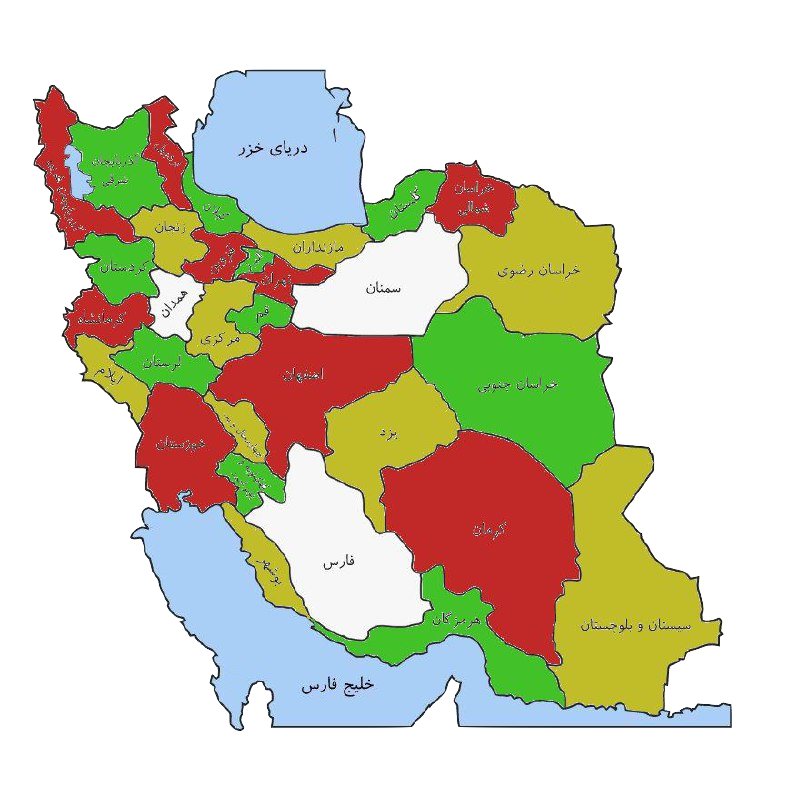
\includegraphics[width=9cm]{/images/problems/43_sol2.png}
\end{center}

21 out of 31 provinces can be colored with 2 colors so that no neighboring provinces are the same color:

\begin{center}
	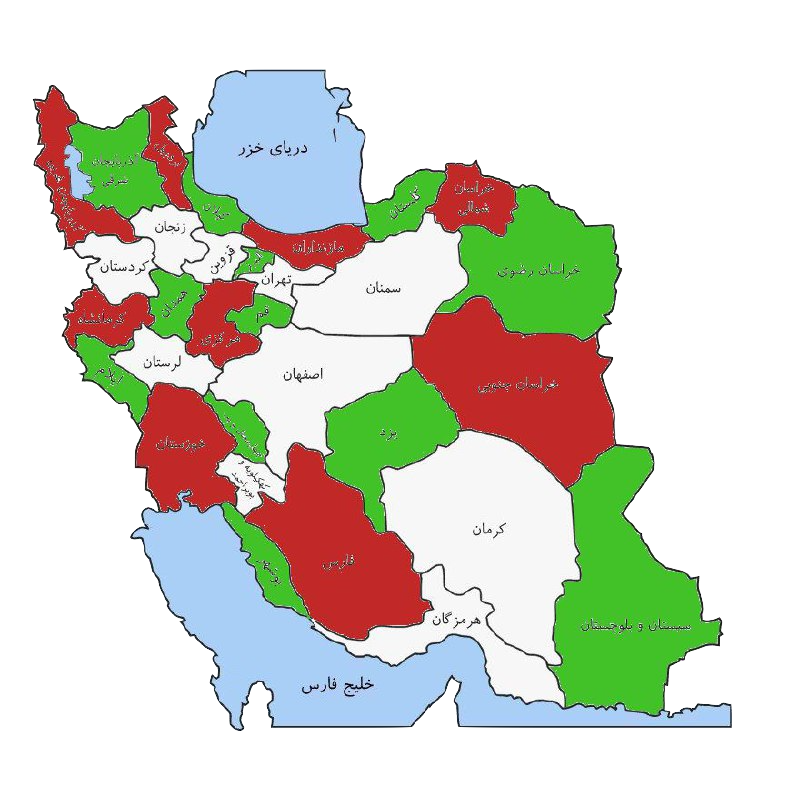
\includegraphics[width=9cm]{/images/problems/43_sol3.png}
\end{center}

It is possible to paint 12 provinces out of 31 with only one color so that no neighboring provinces are the same color (in fact, this is the largest subset of provinces that doesn't contain any neighbors):

\begin{center}
	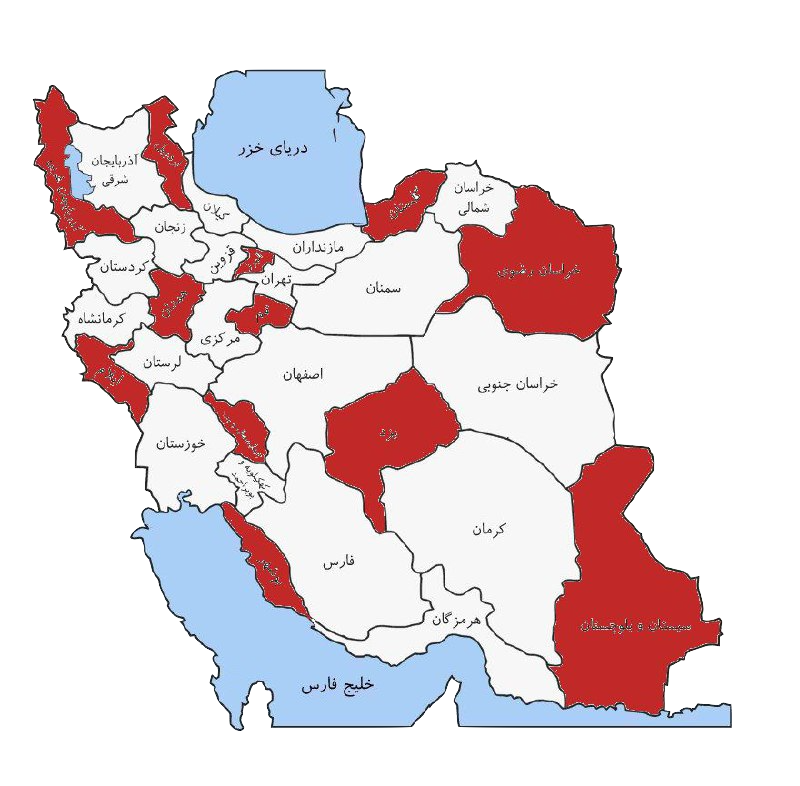
\includegraphics[width=9cm]{/images/problems/43_sol4.png}
\end{center}

\end{solution}
